% !TEX encoding = UTF-8 Unicode
%!TEX root = thesis.tex
% !TEX spellcheck = en-US
%%=========================================
\chapter{Interactive Ontology Matching}

We list here our objectives for an interactive mechanism for matching ontologies
that can assist users in a user feedback loop kind of system:
\begin{itemize}
	\item Show candidate mappings for validation to the users;
          candidate mappings are determined by automatic matching algorithms.
	\item Register the validation choices made by the users..
	\item Allow for class and property navigation to assist users
          in their validation decisions.
	\item Allow users to search for a specific class and navigate
          through the classes.
	\item Support the creation of new mappings that are missed by the automated process.
\end{itemize}


%%=========================================
\section{Interactive Workflow} % (fold)
\label{sub:ambiguous_selection}
Because automatic matching methods do not always provide complete or
correct mappings, the combination of user validation with the
automatic methods can lead to better results than the automatic
methods alone. 

The interactive workflow is shown in
Figure~\ref{fig:workflow}. There exists a user feedback loop (UFL)
approach, in that the results provided by the user are fed back into
the matching process. %\marginpar{need full description using text}
%[need more detail here?]

\begin{figure*}[!ht]
	\centering
	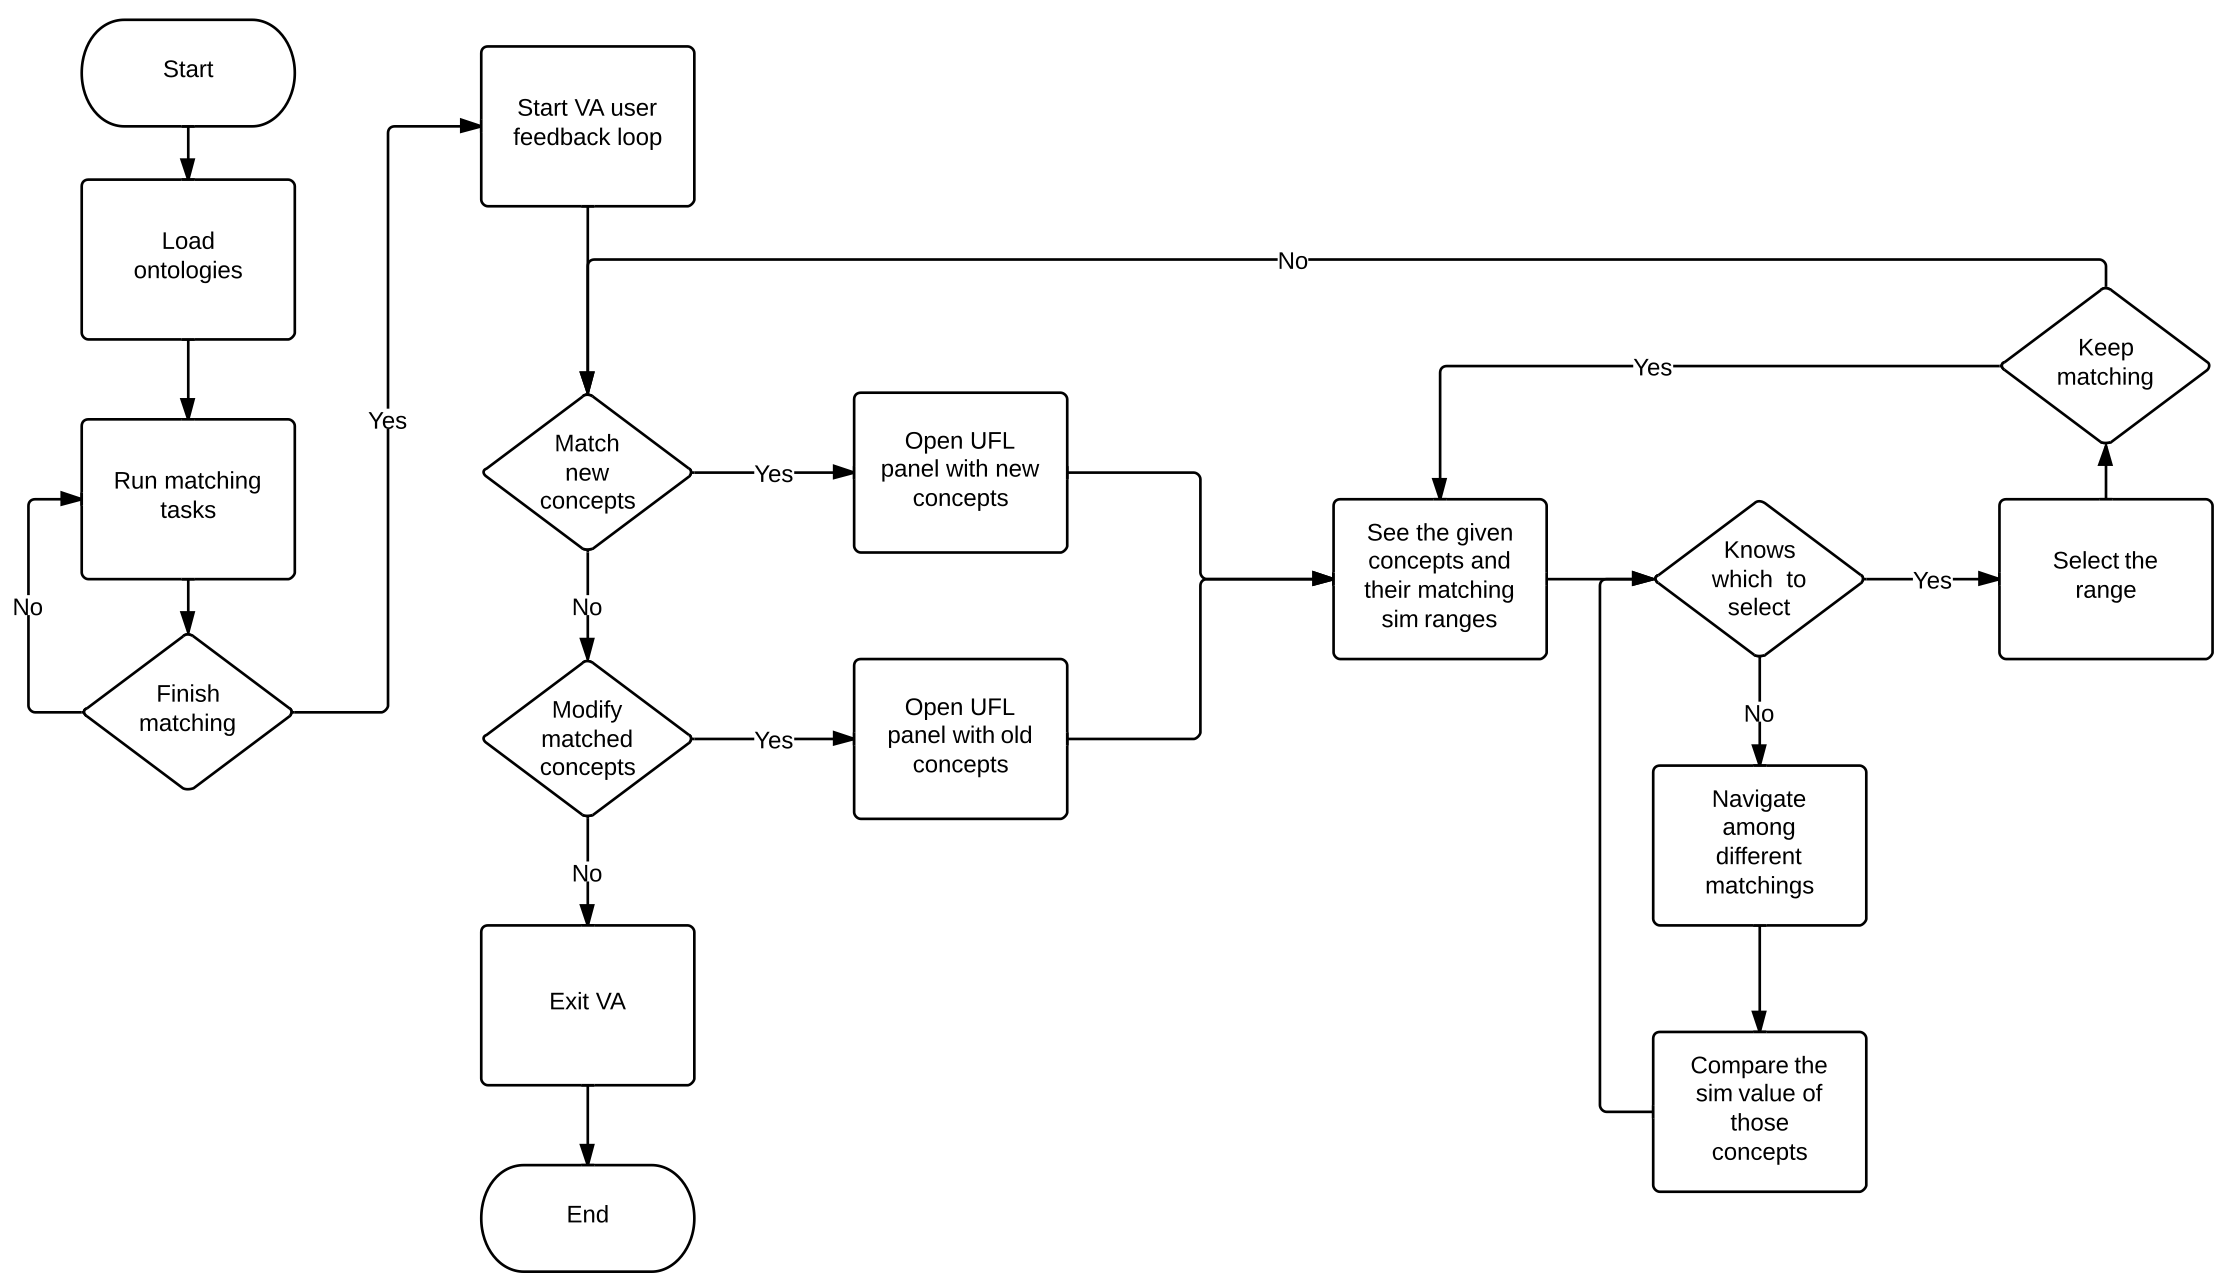
\includegraphics[width=6.5in]{pics/flow.png}
	\caption{Workflow of the interactive process.}
	\label{fig:workflow}
\end{figure*}


\section{User Interface}

The user interface must display one or more mappings to be validated
by users. When showing more than one mapping, users will be asked to
choose one among them. The similarity information among classes is the basis for the
users to make their decisions, which we will supplement with
information about the properties of those classes.

Figure~\ref{fig:url_degisn} shows the design of the panel that enables
the intervention of the users.

\begin{figure}[htb]
	\centering
	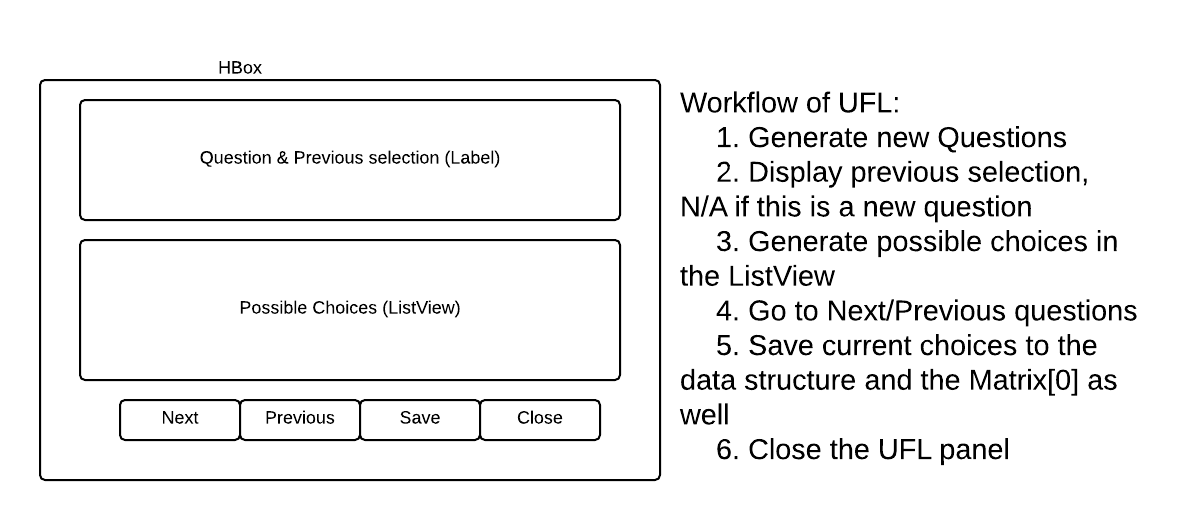
\includegraphics[width=3.5in]{pics/VA_UFL_Design.png}
	\caption{User interface schematic representation.}
	\label{fig:url_degisn}
\end{figure}

Figure~\ref{fig:ambiguous_selection} shows the interface where the
users can select their choice when presented with several possibilities.


\begin{figure}[htb]
	\centering
	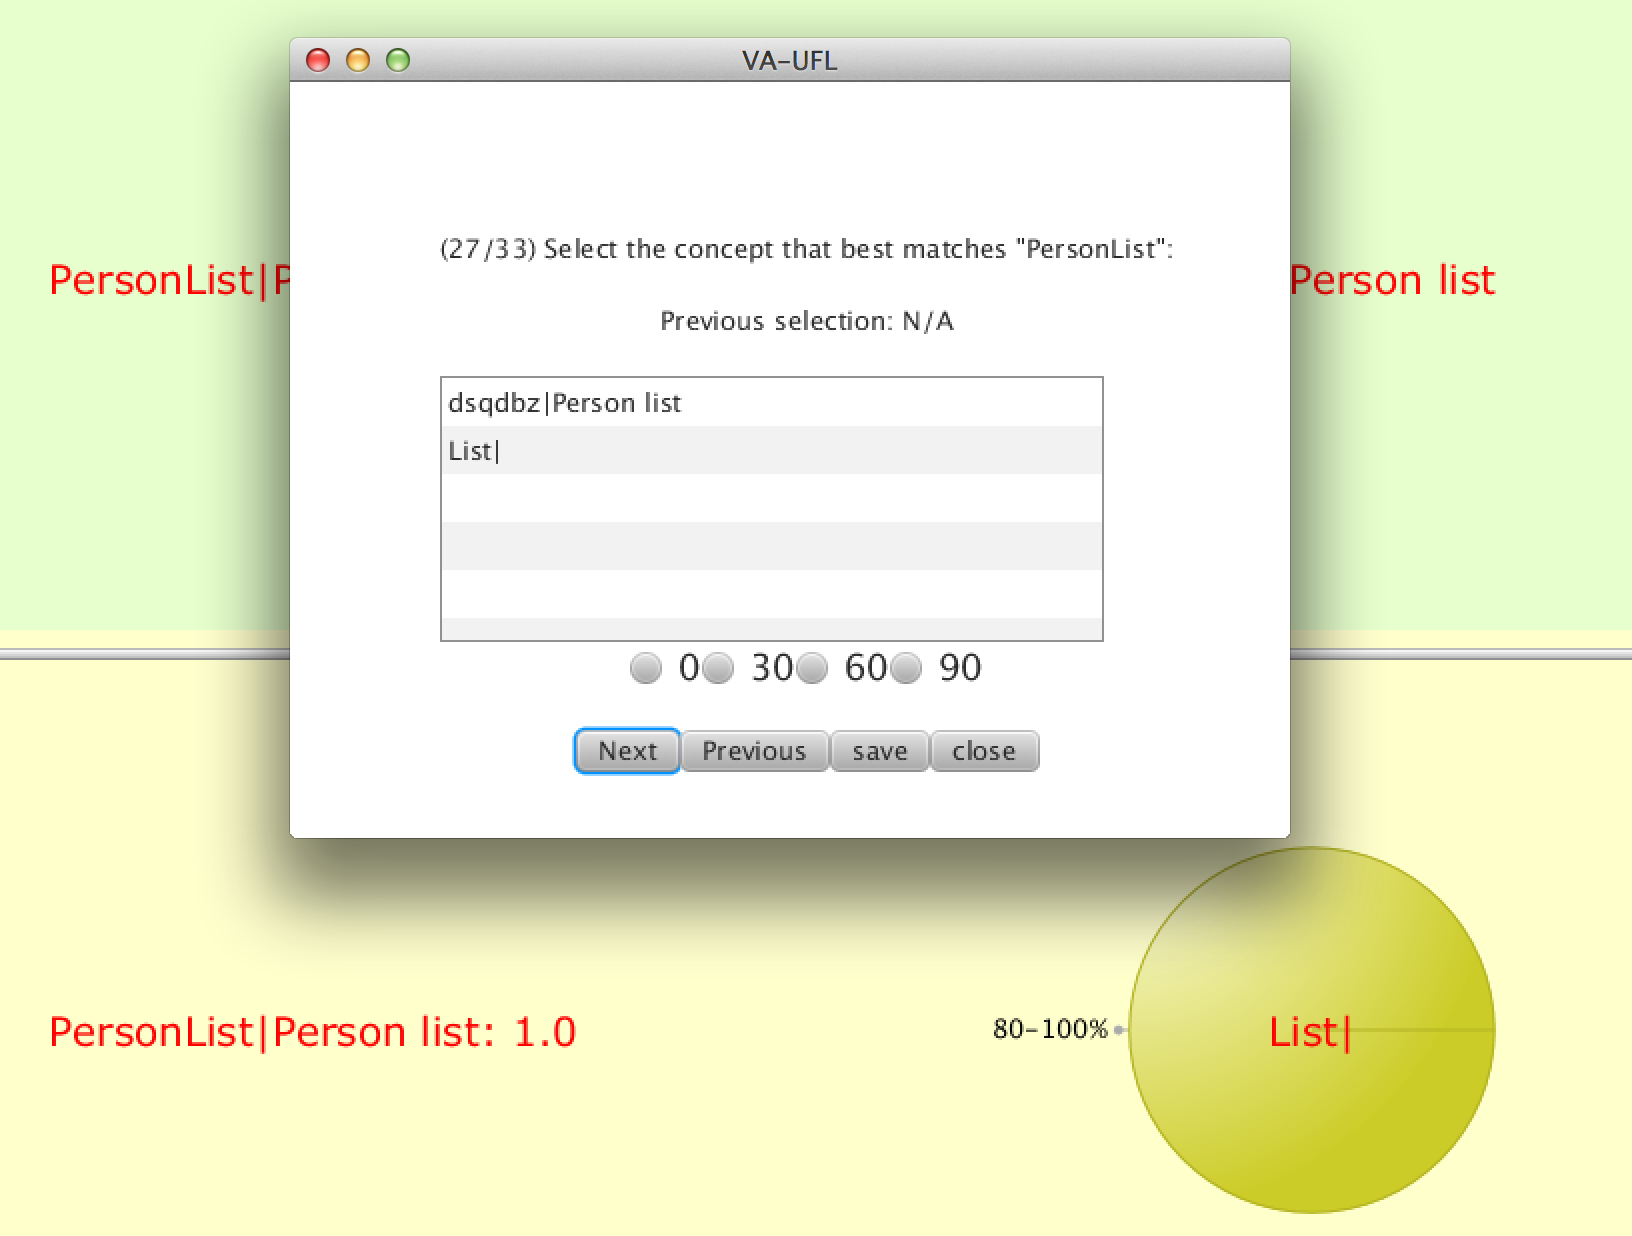
\includegraphics[width=3.5in]{pics/ufl.png}
	\caption{Selection of mappings.}
	\label{fig:ambiguous_selection}
\end{figure}

%%=========================================
\section{Property Clustering} % (fold)
\label{sub:property_clustering}
Falcon-AO~\cite{hu2008falcon} is a practical ontology matching system
with acceptable to good performance and a number of remarkable
features. PBM (Partition-based block matching) is one of the
distinguishing features of Falcon-AO and it is a divide-and-conquer
method for partition-based block matching that is practically
applicable to large class hierarchies. Based on both structural
affinities and linguistic similarities, two large class hierarchies
are partitioned into small blocks. Then, blocks from different
hierarchies are matched based on the relatedness between concepts
called {\it anchors\/} for which similarity values are high. PBM
performs clustering based on structural proximity, for example the
distance between classes in the class hierarchy, and the overlapping
between the domains of properties of a class. In our user feedback
loop strategy when choosing among mappings, we can take the clustering
idea as a reference. When comparing two matching results generated by
different matching algorithms, we therefore not only provide their
matching similarities but also the properties that share the same
domain. In this way, users will be able to see more valuable
information. PBM generates clusters based on the overlapping between
the domains of the properties of both classes. %, in our user feedback loop we use the same idea to make clusters to help user better match the concepts by using their knowledge.\\

We provide an example in Figure~\ref{fig:property_clustering}. We use
the OAEI ontologies for the conference track for the purposes of this
testing. We first load two ontologies, edas.owl (source ontology) and
ekaw.owl (target ontology) and we discover that there are two possible
mappings: 
\begin{itemize}
\item ConferenceEvent maps to Event with matching confidence 0.79,
  using the Parametric String matcher. 
\item ConferenceEvent matches to Conference with matching confidence
  0.61, using the Vector-based Multi-word Matcher (VMM)~\cite{cruz-oaei-2009}.
\end{itemize}

In the reference alignment the correct matching shows as: 
\begin{itemize}
\item ConferenceEvent matches to Conference with matching confidence 1.00 
\end{itemize}
Before asking users to make choices, we generate floating panels to
show users the properties. As we can see from
Figure~\ref{fig:property_clustering}, concept {\it ConferenceEvent\/}
has properties {\it hasAttendee}, {\it hasEndDateTime}, {\it
  hasLocation}, {\it hasProgramme}, and {\it hasStartDateTime}, which
have the same domain as ConferenceEvent; concept Event has properties
{\it eventOnList}, {\it hasEvent}, {\it heldIn}, {\it organisedBy},
and {\it partOfEvent}, which have the same domain as Event; for the
{\it Conference\/} concept, no properties were found.
%\marginpar{picture to be remade}

\begin{figure}[htb]
	\centering
	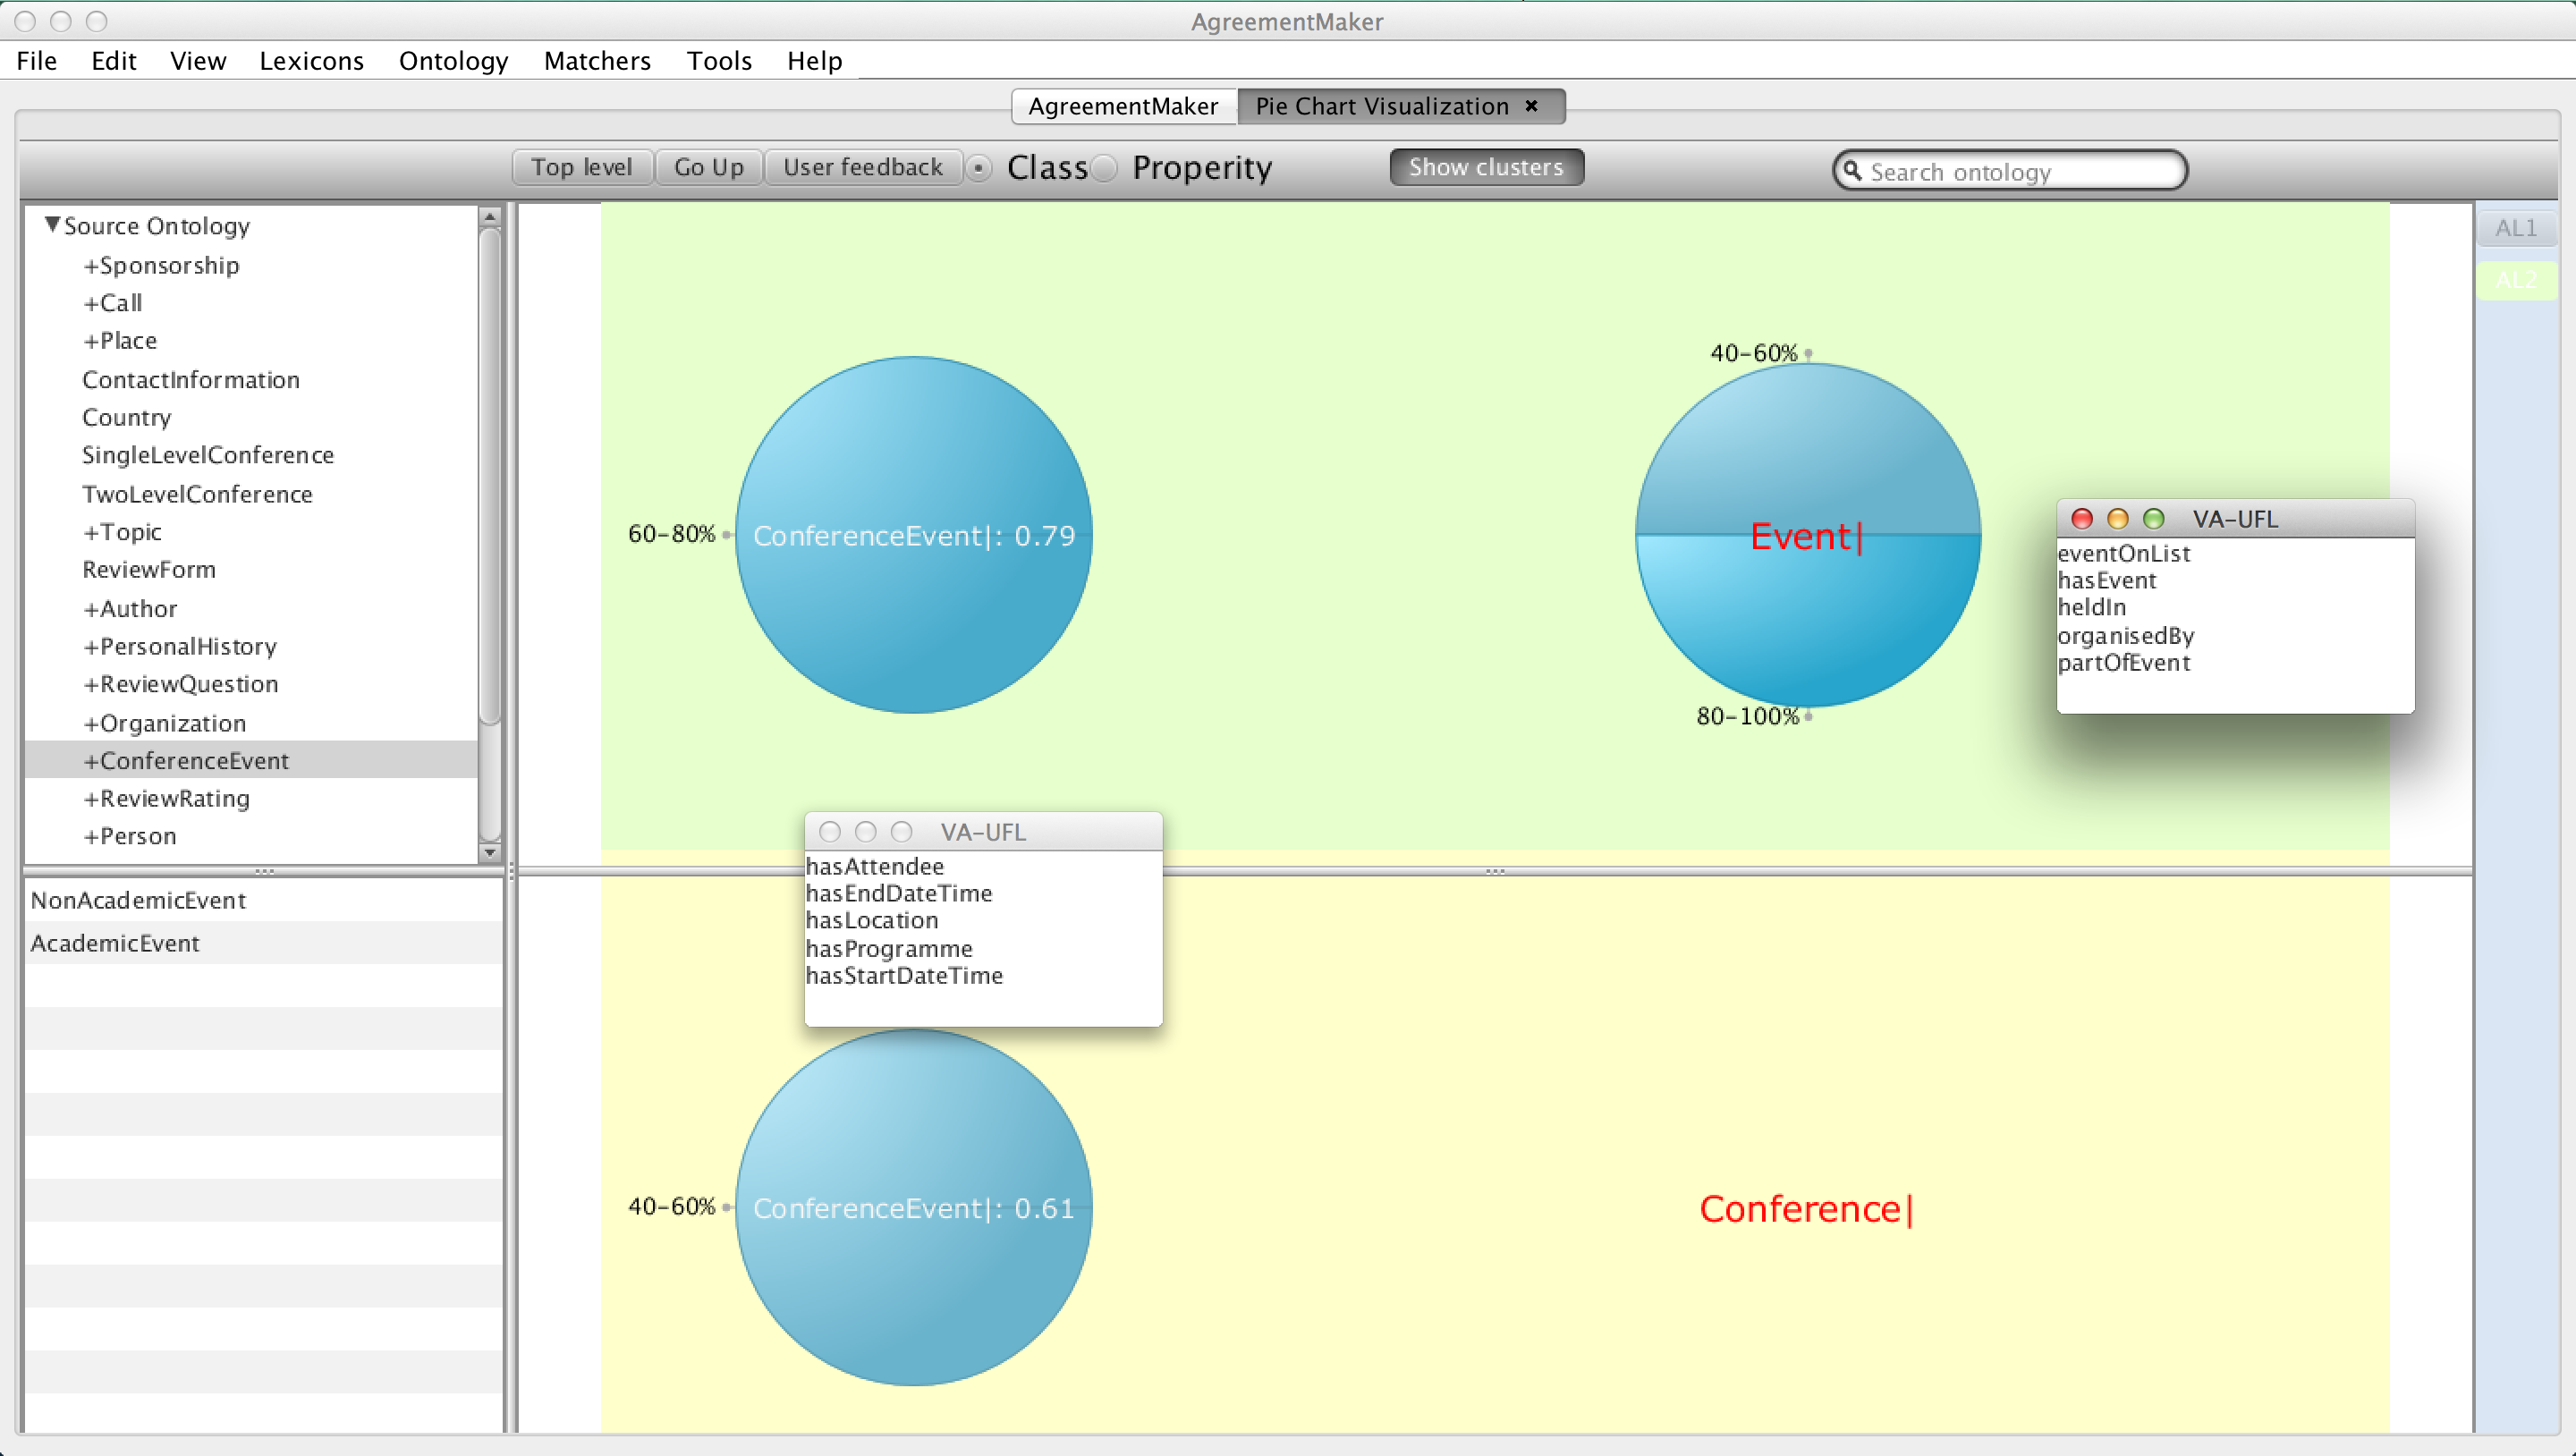
\includegraphics[width=6.5in]{pics/property_cluster.png}
	\caption{Property clustering.}
	\label{fig:property_clustering}
\end{figure}

%%=========================================
\section{Integration with AgreementMaker} % (fold)
\label{sub:integrating_with_agreementMaker}

Using the AgreenmentMaker system, the source and target ontologies are
visualized side by side using a tree paradigm. The control panel (see
Figure~\ref{fig:integrating}) allows users to run a variety of
matchers. In this example, two automatic matchers have been activated (the Parametric String matcher and
the Vector-based Multi-word Matcher) in addition to manual
matching. The picture depicts the display of the two ontologies and the mappings obtained in this way.

\begin{figure}[htb]
	\centering
	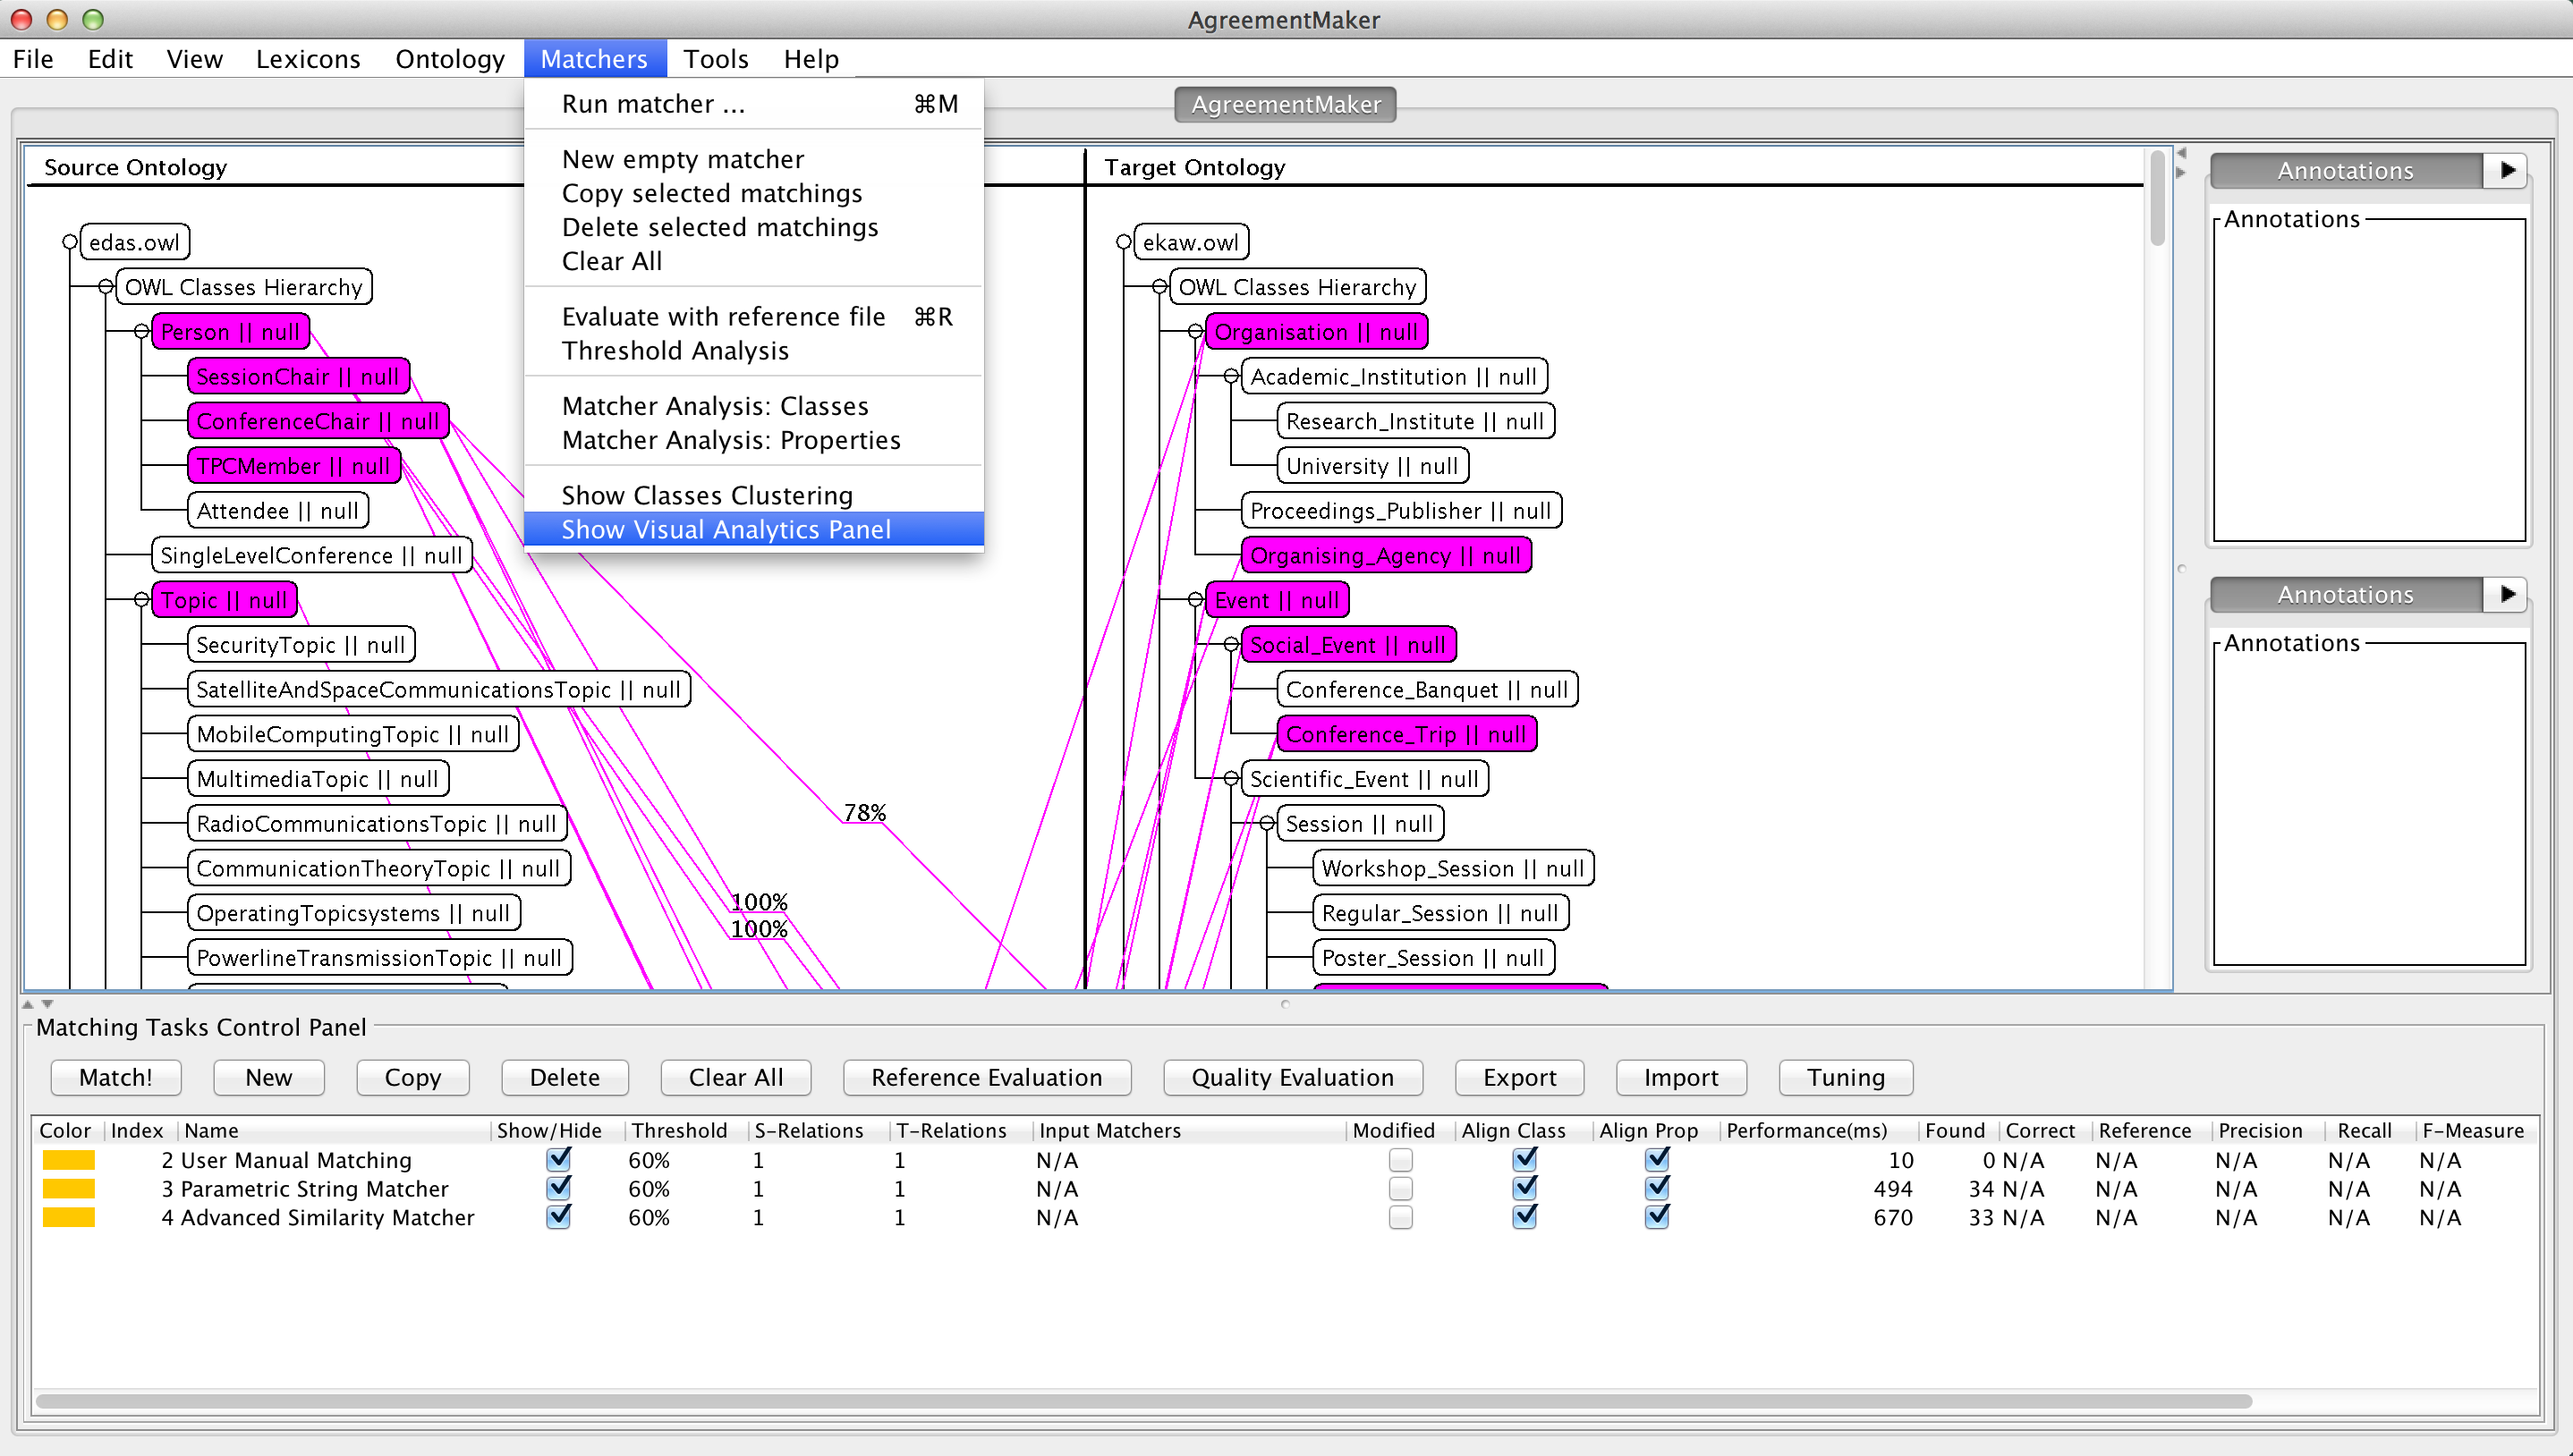
\includegraphics[width=6.5in]{pics/Integrate.png}
	\caption{Integration with AgreementMaker.}
	\label{fig:integrating}
\end{figure} 

Every set of mappings in AgreementMaker is represented by the
MatchingTask class. The MatchingTask class contains the following
elements: a matching algorithm, its associated parameters (e.g.,
the similarity threshold), and the mappings produced by the execution
of the matcher. 

To open our visualization system, users can select the “Pie Chart
Visualization” tab of the drop down menu, as shown in the Figure. The
key point in the integration of the pie chart visualization with AgreementMaker is that we pass all the MatchingTask instances from AgreementMaker to the pie chart visualization.

After selecting the “Pie Chart Visualization” tab, another tab will
show up and the pie charts will be initialized automatically (see
Figure~\ref{fig:updated_main_panel}). Users can easily switch between the
tree and pie chart visualizations by clicking on the available tabs at
the top of the display.

%In AgreementMaker, after executing the loaded algorithms, we first
%select the matrix that contains the resulting mappings with the
%highest matching similarity confidence. We make a copy of this matrix
%and regard it as the user defined matrix. Then we start the user
%feedback loop process and modify the user defined matrix with user
%selected alignments.  %\marginpar{picture to be replaced}

%In AgreenmentMaker System, each matching algorithm is stored in a MatchingTask data structure. As shown in \ref{fig:integrating}, after loading the two ontology files (e.g. eras.owl and ekaw.owl), we run two matchers, which are the Parametric String matcher and the Vector-based Multi-word Matcher (VMM). Then we can see three rows in the "Matching Tasks Control Panel". The first row is the "User Manual Matching", which is an empty MatchingTask structure by default. The next two rows are the two matchers we loaded.

%The next step is to click on the "Show Visulization System" in the drop down menu. Once clicked, the MatchingTask data structures generated by the two matchers will be loaded into our visualization system.

%After loading all the MatchingTask data structures, the visualization system will first select the MatchingTask with the highest matching confidence value and make a copy of it. We name this copy the "User defined" mappings and once the user feedback loop process starts, we modify the this mapping according to the user selected alignments. 
%\marginpar{1) Not clear. 2) Also, pic highlights
%wrong alg.}


